\documentclass[11pt]{article}
\usepackage[margin=1in]{geometry}
\usepackage[T1]{fontenc}
\usepackage[utf8]{inputenc}
\usepackage{lmodern}
\usepackage{microtype}
\usepackage{hyperref}
\usepackage{booktabs}
\usepackage{longtable}
\usepackage{array}
\usepackage{graphicx}
\usepackage{amsmath}
\usepackage{tikz}
\usepackage{pgfplots}
\usepackage[numbers]{natbib}

\usetikzlibrary{arrows.meta,positioning,shapes.geometric,calc}
\pgfplotsset{compat=1.18}

\hypersetup{
  colorlinks=true,
  linkcolor=blue,
  citecolor=blue,
  urlcolor=blue
}

\title{Toward Verified Long-Horizon Language Agents:\\Real-Model Evidence for Hybrid Memory, Bounded State, Planning, Integrated Execution, and Latent Predictive Dynamics}
\author{Kunj Rathod\\School of Computing, University of Utah\\\texttt{kunj.rathod@utah.edu}}
\date{}

\begin{document}
\maketitle

\begin{abstract}
Transcript-only language agents are a bad substrate for long-horizon autonomy because they mix memory, working state, action selection, and state commitment into one growing prompt. We test a modular alternative with six laptop-scale experiments: hybrid memory retrieval on 1,977 LoCoMo questions, bounded-workspace reconstruction over eight real arXiv abstracts, stronger open-weight planning conditions in a key-door world, an integrated memory--workspace--verification loop on the same literature task, an embedding-space latent dynamics baseline over 9,512 transitions, and an architectural comparison between an MLP, a causal transformer, and a minimal linear recurrent unit. Hybrid retrieval improves LoCoMo Hits@5 from 0.4385 (TF-IDF) to 0.4891; bounded workspace reduces cumulative prompt load by 57.96\%; transcript-only planning still fails even after scaling from distilgpt2 to Qwen2.5-1.5B-Instruct and adding a 3-shot chain-of-thought prompt, while verifier-backed search solves every task; the integrated pipeline cuts prompt load from 62,536 to 25,310 characters, raises schema pass rate from 0.625 to 1.0, and flags two malformed commits before they enter trusted state; and latent prediction remains geometrically easy but symbolically brittle, with one-step cosine 0.9989 but only 0.0981 local Top-1 decode. On the sequential latent task, a minimal linear recurrent proxy slightly exceeds the causal transformer on local decode accuracy while using fewer parameters, suggesting that bounded-state agent architectures benefit from explicit memory, bounded reconstruction, and verification more than from ever-larger transcript policies.
\end{abstract}

\section{Introduction}
Large language models are increasingly deployed as agents rather than pure text generators. In practice, however, many ``LLM agents'' are still little more than autoregressive policies wrapped around tools and prompts. This design inherits three deep failure modes. First, persistent knowledge is weak: once context falls out of the prompt window, the agent either forgets or must recover it through ad hoc retrieval. Second, long-horizon execution is unstable because the prompt grows with the transcript rather than with task-relevant state. Third, action selection is probabilistic while the environments in which these agents operate often have hard constraints, irreversible operations, and externally verifiable transition rules.

A growing literature points beyond this transcript-centric paradigm. JEPA-style models shift predictive learning from raw token or pixel reconstruction to latent target prediction, encouraging abstraction over surface form \citep{vljepa2025, vjepa22025}. World-model reinforcement learning has long shown that latent dynamics can support planning more efficiently than observation-space reasoning alone \citep{planet2018, dreamerv32023}. Agent memory systems such as MemGPT and Hindsight argue for hierarchical or typed memory rather than flat stateless retrieval \citep{memgpt2023, hindsight2025}. Long-horizon agent frameworks increasingly externalize persistent state into files or workspaces to avoid unbounded context growth \citep{infiagent2026}. Verification-oriented frameworks such as ReAct, LATS, and ToolGate show that language-based proposal should be separated from execution and state commitment \citep{react2023, lats2023, toolgate2026}.

The central claim of this paper is modest but testable: long-horizon agent reliability improves when language is embedded inside an explicit architecture for memory, bounded workspace state, transition modeling, and verifier-mediated commits. This is a systems paper rather than a frontier-model paper. We deliberately use real benchmark data, real open-weight models, and a commodity laptop so the architectural effect can be tested before spending serious compute.

\paragraph{Code availability.} Experiments, results, and paper source are available at \href{https://github.com/rathodkunj2005/verified-long-horizon-agents}{github.com/rathodkunj2005/verified-long-horizon-agents}.

\paragraph{Contributions.}
\begin{enumerate}
    \item We formalize a modular architecture for long-horizon language agents that separates language interaction from persistent memory, bounded workspace state, transition modeling, and verifier-mediated trusted-state commits.
    \item We evaluate six hypotheses with reproducible experiments that all run on an Apple M1 Pro laptop: (1) LoCoMo hybrid retrieval, (2) bounded-workspace literature synthesis, (3) stronger open-weight planning baselines including Qwen2.5-1.5B-Instruct and a 3-shot CoT prompt, (4) embedding-space latent dynamics, (5) an integrated memory+workspace+verification pipeline over the same literature workflow, and (6) a sequential architectural comparison between MLP, causal transformer, and minimal LRU predictors.
    \item We show that the strongest empirical gains come from architectural discipline rather than raw language-model scaling: hybrid memory beats dense retrieval, bounded state curbs prompt growth, verification solves planning where greedy decoding fails, and recurrent compression remains competitive with causal self-attention for short-horizon agent state prediction.
\end{enumerate}

\section{Problem Setting and Design Requirements}
We consider an agent operating over turns $t = 1, 2, \ldots$ with four persistent objects:
\begin{itemize}
    \item a task state $z_t$ that summarizes current goals, hypotheses, and environment-relevant latent information,
    \item a memory bank $M_t$ containing retained world facts, experiences, and derived summaries,
    \item a bounded prompt context $C_t$ constructed from a snapshot of state plus retrieved memory and a short recent window,
    \item a verifier $V$ that determines whether a proposed action may be executed and whether its result may update trusted state.
\end{itemize}
The language model produces proposals conditioned on $C_t$. The environment and verifier determine whether those proposals become committed transitions.

This framing yields five design requirements.
\begin{description}
    \item[R1: Persistence.] Information relevant across long horizons should be stored outside the prompt and updated over time.
    \item[R2: Boundedness.] Prompt construction should scale with state complexity, not transcript length.
    \item[R3: Verifiability.] State updates should be gated by executable checks or trusted transition rules.
    \item[R4: Predictive state.] The architecture should support compact internal prediction for planning without decoding every intermediate state into text.
    \item[R5: Practicality.] The design should admit useful experiments on commodity hardware, so the systems hypothesis can be tested before large-scale training.
\end{description}

\section{Related Work}
\subsection{Language agents and cognitive architectures}
ReAct established the now-standard reasoning-and-acting loop for LLMs with tools \citep{react2023}. LATS extended this framing with explicit tree search and environment feedback \citep{lats2023}. OpenAgents emphasized deployment-oriented language agents in real usage settings \citep{openagents2023}. CoALA organized these trends under a broader cognitive-architecture perspective, arguing that language agents should be understood as systems with modular memory and action interfaces rather than single-pass prompt programs \citep{coala2023}. The present work is closest in spirit to CoALA, but it tests a narrower thesis about memory, bounded state, verification, and lightweight predictive state.

\subsection{Persistent memory for agents}
MemGPT introduced an operating-system analogy for hierarchical memory management in LLM systems \citep{memgpt2023}. LoCoMo provided a benchmark specifically designed to measure very long-term conversational memory beyond short-session chat \citep{locomo2024}. Hindsight proposed a more structured memory substrate with separate networks for facts, experiences, summaries, and beliefs, together with retain/recall/reflect operations \citep{hindsight2025}. Our retrieval experiment is directly motivated by this line of work: the interesting question is not whether retrieval helps in the abstract, but which retrieval mixture remains robust on long-horizon conversational memory.

\subsection{World models and latent predictive state}
PlaNet and Dreamer demonstrated that planning over latent dynamics can outperform observation-space planning in reinforcement learning settings \citep{planet2018, dreamerv32023}. More recently, JEPA-style representation learning has pushed this idea into self-supervised multimodal modeling. VL-JEPA predicts target text embeddings rather than generating text autoregressively, while V-JEPA 2 and its action-conditioned extension show that latent predictive architectures can support physical planning from large-scale video pretraining \citep{vljepa2025, vjepa22025}. We do not train a V-JEPA-scale model here. Instead, we test a smaller claim: if agent state is embedded in a latent space, how far does simple next-embedding prediction get before exact symbolic decoding becomes the bottleneck?

\subsection{Verification and bounded execution}
InfiAgent argues that persistent workspace state should live outside the transcript, with each reasoning step reconstructed from a bounded snapshot \citep{infiagent2026}. ToolGate formalizes tool use through preconditions and postconditions, preventing hallucinated outputs from directly contaminating trusted state \citep{toolgate2026}. Our planning and integrated-pipeline experiments follow the same interface logic: language may propose or rank actions, but legality and commit rights are delegated to explicit mechanisms.

\subsection{State space models and recurrent alternatives}
Recent sequence-model work makes it reasonable to ask whether bounded agent state is better matched to recurrent compression than to attention over an ever-growing token tape. Mamba uses selective state spaces to obtain linear-time sequence modeling with strong long-context performance \citep{mamba2023}. Griffin mixes gated linear recurrences with local attention and is especially relevant here because it offers a tractable recurrent alternative for language modeling on commodity hardware \citep{griffin2024}. We do not implement full Mamba because its practical advantage depends on hardware-aware CUDA kernels unavailable on Apple Silicon; instead we use a minimal LRU-style proxy to test the architectural question in a controlled setting.

\section{Architecture}
Figure~\ref{fig:architecture} shows the architecture studied in this paper. The claim is not that any individual box is novel; the claim is that reliable long-horizon agents need clean separation between these interfaces.

\begin{figure}[t]
\centering
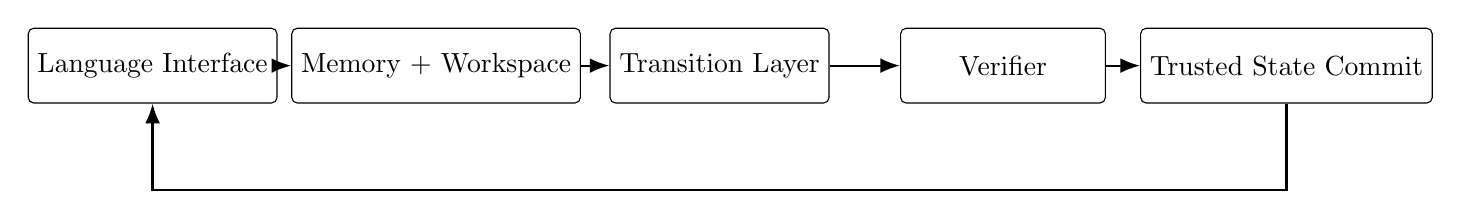
\begin{tikzpicture}[
  box/.style={draw, rounded corners=2pt, minimum width=2.6cm, minimum height=0.95cm, align=center},
  arrow/.style={-{Latex[length=2.5mm]}, thick}
]
\node[box] (lang) at (0,0) {Language Interface};
\node[box] (mem) at (3.6,0) {Memory + Workspace};
\node[box] (trans) at (7.2,0) {Transition Layer};
\node[box] (ver) at (10.8,0) {Verifier};
\node[box] (commit) at (14.4,0) {Trusted State Commit};

\draw[arrow] (lang.east) -- (mem.west);
\draw[arrow] (mem.east) -- (trans.west);
\draw[arrow] (trans.east) -- (ver.west);
\draw[arrow] (ver.east) -- (commit.west);
\draw[arrow] (commit.south) |- ++(0,-1.1) -| (lang.south);
\end{tikzpicture}
\caption{Publication-style interface diagram for the proposed agent architecture. Language proposes; memory and workspace reconstruct bounded context; the transition layer predicts or enumerates futures; the verifier authorizes trusted commits; and committed state feeds the next interaction turn.}
\label{fig:architecture}
\end{figure}

\paragraph{Language interface $L(C_t) \rightarrow a_t$.} Given bounded context $C_t$, the language model proposes an action, a search query, a summary, or a candidate plan. This module is optimized for interaction and semantic compression, not trusted state mutation.

\paragraph{Memory and workspace $R(M_t, z_t, h_t) \rightarrow C_t$.} The retrieval constructor takes memory $M_t$, compact state $z_t$, and a short recent history $h_t$ and returns bounded context $C_t$. This is where R1 and R2 live: memory persists outside the prompt, and context reconstruction remains bounded.

\paragraph{Transition model $T(z_t, a_t) \rightarrow \hat{z}_{t+1}$ or $\mathcal{N}(z_t)$.} This module either predicts latent next state or enumerates legal successors. It can be learned, symbolic, or hybrid. R4 is enforced here.

\paragraph{Verifier $V(z_t, a_t, o_{t+1}) \rightarrow \{\mathrm{commit}, \mathrm{reject}\}$.} The verifier checks whether a proposed action is legal and whether its observed result may update trusted state. If verification fails, the language module may repair or replan, but no state is silently committed.

\section{Experimental Hypotheses and Setup}
We test six hypotheses.

\paragraph{H1.} Hybrid retrieval over persistent memory outperforms dense retrieval alone on long-horizon conversational memory questions.

\paragraph{H2.} Reconstructing prompts from bounded workspace state reduces cumulative context load on a real-data iterative workflow.

\paragraph{H3.} Small open-weight language models remain unreliable standalone planners in constrained environments even after modest scaling and 3-shot CoT prompting, but the same models can be embedded inside verifier-backed search.

\paragraph{H4.} Learning next-state prediction in latent embedding space is geometrically easy but insufficient for exact long-horizon symbolic decoding without additional structure.

\paragraph{H5.} Wiring memory retrieval, bounded workspace reconstruction, and verification into one loop improves end-to-end execution quality over transcript-only or partially modular baselines.

\paragraph{H6.} For sequential agent state prediction, a linear recurrent architecture matches or exceeds causal self-attention in decode accuracy at lower parameter cost on short-horizon episodes.

\paragraph{Compute environment.} All experiments run on a MacBook Pro with Apple M1 Pro, 16 GB unified memory, Python 3.11, and PyTorch on MPS unless otherwise noted. The recurrent architectural comparison runs on CPU because the minimal LRU proxy uses plain PyTorch complex arithmetic rather than specialized kernels. All requested planning conditions completed locally; no model exceeded the 4 GB skip threshold.

\subsection{Experiment 1: LoCoMo retrieval with real embeddings}
We use the publicly released \texttt{locomo10.json} subset from the LoCoMo project \citep{locomo2024}. The resulting evaluation contains 1,977 question-answer pairs and 5,882 dialogue turns. Each question includes gold evidence references to one or more dialogue turns.

We flatten each conversation into memory items indexed by dialogue identifier and compare three retrieval methods:
\begin{itemize}
    \item \textbf{TF-IDF}: lexical retrieval using \texttt{TfidfVectorizer},
    \item \textbf{Dense}: sentence embeddings from \texttt{all-MiniLM-L6-v2},
    \item \textbf{Hybrid}: reciprocal-rank fusion of lexical and dense rankings.
\end{itemize}
Metrics are Hits@1, Hits@5, Hits@10, MRR, and nDCG@10, where a hit is counted if any gold evidence item is retrieved.

\subsection{Experiment 2: bounded-workspace reconstruction on a real-data workflow}
To test R2 without falling back to a toy transcript simulator, we construct a deterministic literature-synthesis loop over eight arXiv abstracts cited in this paper. At each step, the workflow ingests one paper title and abstract, writes a structured note containing the title, a claim sentence, and extracted keywords, and updates the persistent workspace. We compare a transcript baseline whose prompt grows with all prior observations and actions against a bounded-workspace baseline whose prompt is rebuilt from the structured workspace plus the two most recent actions.

\subsection{Experiment 3: stronger open-weight planning with verification}
We construct a symbolic $5\times5$ key-door gridworld. Tasks require navigating to a goal while respecting walls and a locked door that can only be opened after acquiring a key. The models are distilgpt2, Qwen2.5-0.5B-Instruct, a 3-shot chain-of-thought prompting condition on Qwen2.5-0.5B-Instruct, and Qwen2.5-1.5B-Instruct. Rather than unconstrained text generation, we score legal action strings under each model.

We compare three planners:
\begin{itemize}
    \item \textbf{Greedy LM}: at each state, choose the highest-probability legal action under the model.
    \item \textbf{LM-scored BFS}: use the model only to order frontier expansions inside a breadth-first search over legal states.
    \item \textbf{Pure BFS}: symbolic breadth-first search without the language-model prior.
\end{itemize}
The key-door setting matters because success depends on maintaining a hidden boolean state, \texttt{has\_key}, across multiple steps. A fluent local continuation can still be wrong if it ignores this state bit.

\subsection{Experiment 4: embedding-space latent dynamics baseline}
We generate 9,512 state transitions from the same symbolic environment. Each state is rendered as a compact textual description and embedded with \texttt{all-MiniLM-L6-v2}. A small MLP receives the current state embedding and an action embedding and is trained to predict the next-state embedding. This is a JEPA-inspired embedding-space baseline, not a claim of VL-JEPA- or V-JEPA-scale training.

We evaluate one-step cosine similarity, global nearest-neighbor decode accuracy, local nearest-neighbor decode accuracy restricted to the same task instance, and rollout cosine similarity over horizons 1, 3, and 5.

\subsection{Experiment 5: integrated memory--workspace--verification pipeline}
To address the obvious reviewer complaint that memory, workspace, and verification were previously tested in isolation, we build a lightweight integrated loop over the same eight abstracts from Experiment 2. At each step, the system first retrieves the most relevant prior note using the hybrid retriever from Experiment 1, then reconstructs the prompt from either the full transcript or a bounded workspace state, then writes a structured note, and finally applies a deterministic schema verifier that checks three conditions: non-empty title, at least one keyword, and non-empty claim sentence. If verification fails in the full pipeline, the step is counted as a failed commit and the note is repaired before it enters trusted state.

We compare three settings: transcript-only, memory+workspace without verification, and the full integrated pipeline. Metrics are cumulative prompt load, schema pass rate, retrieval overlap (cosine similarity $> 0.4$ between the retrieved prior note and the current abstract), and the number of failed commits flagged by the verifier.

\subsection{Experiment 6: architectural comparison for latent state prediction}
Using the same 9,512 transitions and \texttt{all-MiniLM-L6-v2} embeddings from Experiment 4, we treat each task instance as a sequence of $(\text{state\_emb}, \text{action\_emb})$ pairs and train three predictors for next-state embedding:
\begin{itemize}
    \item \textbf{Architecture A: MLP control.} The non-sequential baseline from Experiment 4, using only the current state-action pair.
    \item \textbf{Architecture B: Causal Transformer.} A 2-layer causal self-attention model with 4 heads, $d_{model}=128$, and learned absolute positional encodings.
    \item \textbf{Architecture C: Minimal LRU.} A single-layer linear recurrent unit with hidden size 128 and diagonal complex recurrence, used as a tractable proxy for Griffin-like recurrent compression \citep{griffin2024}.
\end{itemize}
We implement the minimal LRU as a tractable proxy for selective-scan state-space architectures; full Mamba-style implementations depend on hardware-aware CUDA kernels unavailable on Apple Silicon \citep{mamba2023}. Evaluation metrics are one-step cosine, local Top-1 and Top-5 decode, rollout cosine at horizons 1, 3, and 5, parameter count, and training time.

\section{Results}
\subsection{Experiment 1: conversational memory retrieval}
\begin{table}[t]
    \centering
    \caption{Retrieval results on 1,977 LoCoMo questions and 5,882 dialogue-turn memories.}
    \begin{tabular}{lccccc}
        \toprule
        Method & Hits@1 & Hits@5 & Hits@10 & MRR & nDCG@10 \\
        \midrule
        TF-IDF & 0.2352 & 0.4385 & 0.5250 & 0.3337 & 0.3513 \\
        Dense MiniLM & 0.1507 & 0.3409 & 0.4294 & 0.2456 & 0.2586 \\
        Hybrid & 0.2190 & 0.4891 & 0.5802 & 0.3426 & 0.3687 \\
        \bottomrule
    \end{tabular}
    \label{tab:retrieval}
\end{table}

\noindent Hybrid Hits@1 falls below TF-IDF because reciprocal-rank fusion dilutes the dominant lexical rank-1 signal when the dense model disagrees at the top position; the gain from hybridization accumulates at Hits@5 and above.

Hybrid retrieval is the correct reading of this result, not ``dense beats lexical.'' Dense retrieval alone underperforms TF-IDF on this LoCoMo subset, likely because conversational memory questions rely heavily on exact names, dates, and temporal details. But hybrid fusion improves Hits@5 by 5.1 points and Hits@10 by 5.5 points over TF-IDF while also improving MRR and nDCG@10, which supports H1.

\begin{figure}[t]
\centering
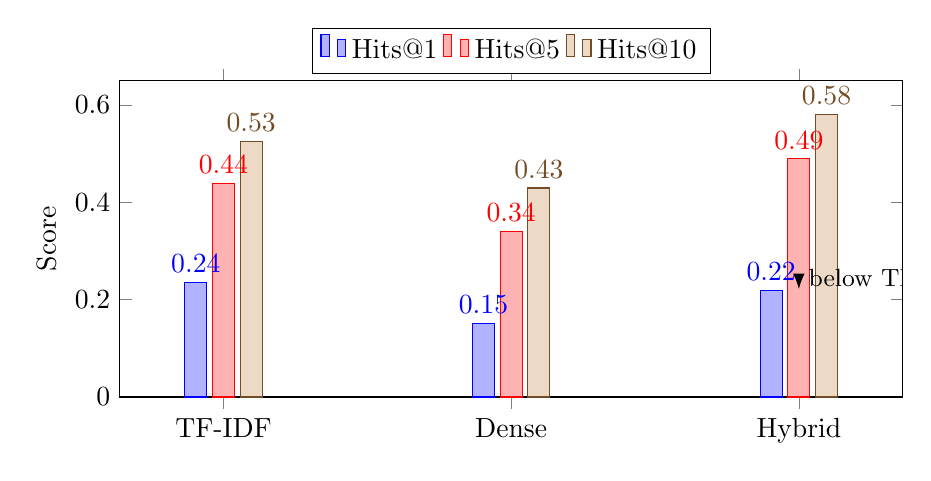
\begin{tikzpicture}
\begin{axis}[
    ybar,
    bar width=8pt,
    width=0.95\linewidth,
    height=5.6cm,
    ymin=0,
    ymax=0.65,
    ylabel={Score},
    symbolic x coords={TF-IDF,Dense,Hybrid},
    xtick=data,
    legend style={at={(0.5,1.02)}, anchor=south, legend columns=3},
    nodes near coords,
    nodes near coords align={vertical},
    enlarge x limits=0.18
]
\addplot coordinates {(TF-IDF,0.2352) (Dense,0.1507) (Hybrid,0.2190)};
\addplot coordinates {(TF-IDF,0.4385) (Dense,0.3409) (Hybrid,0.4891)};
\addplot coordinates {(TF-IDF,0.5250) (Dense,0.4294) (Hybrid,0.5802)};
\legend{Hits@1, Hits@5, Hits@10}
\node[anchor=west, font=\small] at (axis cs:Hybrid,0.245) {below TF-IDF at rank 1};
\draw[-{Latex[length=2mm]}, thick] (axis cs:Hybrid,0.24) -- (axis cs:Hybrid,0.221);
\end{axis}
\end{tikzpicture}
\caption{LoCoMo retrieval metrics grouped by method. Hybrid underperforms TF-IDF at Hits@1 but gains substantially at Hits@5 and Hits@10.}
\label{fig:retrieval-bars}
\end{figure}

\subsection{Experiment 2: bounded workspace reconstruction}
\begin{table}[t]
    \centering
    \caption{Bounded-workspace results on an eight-document literature-synthesis workflow over real arXiv abstracts.}
    \begin{tabular}{lcc}
        \toprule
        Metric & Full transcript & Bounded workspace \\
        \midrule
        Final prompt size (chars) & 14,346 & 4,770 \\
        Cumulative prompt load (chars) & 65,558 & 27,561 \\
        Title coverage & 1.0 & 1.0 \\
        Keyword coverage & 1.0 & 1.0 \\
        \bottomrule
    \end{tabular}
    \label{tab:workspace}
\end{table}

The bounded-workspace condition reduces cumulative prompt load by 57.96\% while preserving complete title and keyword coverage. This is still a lightweight workflow rather than a full agent benchmark, but it is no longer a toy transcript-growth demo. It directly supports H2.

\begin{figure}[t]
\centering
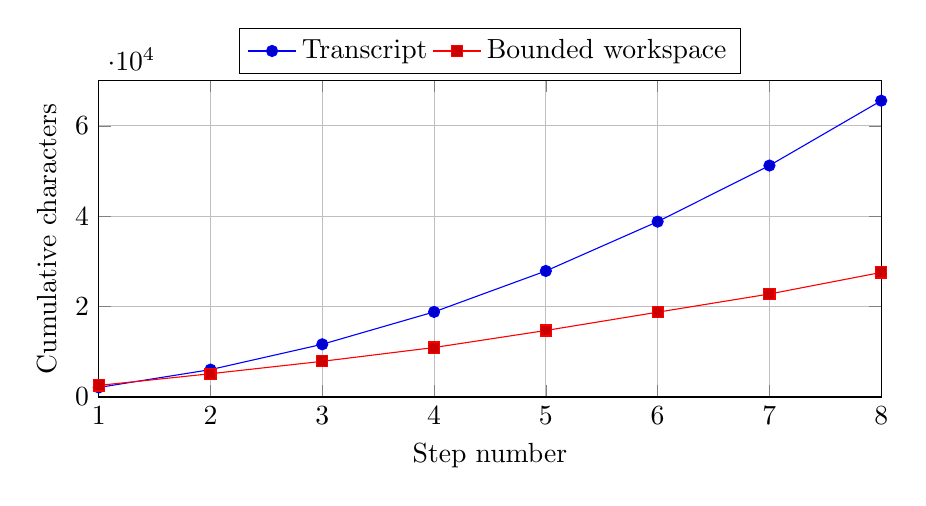
\begin{tikzpicture}
\begin{axis}[
    width=0.95\linewidth,
    height=5.6cm,
    xmin=1, xmax=8,
    ymin=0, ymax=70000,
    xlabel={Step number},
    ylabel={Cumulative characters},
    xtick={1,2,3,4,5,6,7,8},
    legend style={at={(0.5,1.02)}, anchor=south, legend columns=2},
    grid=major
]
\addplot+[mark=*] coordinates {(1,2113) (2,6061) (3,11667) (4,18829) (5,27888) (6,38801) (7,51212) (8,65558)};
\addplot+[mark=square*] coordinates {(1,2567) (2,5153) (3,7899) (4,10949) (5,14720) (6,18768) (7,22791) (8,27561)};
\legend{Transcript, Bounded workspace}
\end{axis}
\end{tikzpicture}
\caption{Cumulative prompt load over eight steps. The bounded workspace changes growth rate rather than merely shaving a constant offset.}
\label{fig:workspace-line}
\end{figure}

\subsection{Experiment 3: stronger open-weight planning with verification}
\begin{table}[t]
    \centering
    \caption{Planning results on constrained gridworld tasks. Caption note: The LM prior does not reduce search expansions relative to pure BFS; its contribution is action ranking only, not search efficiency.}
    \begin{tabular}{lccc}
        \toprule
        Planner & Success rate & Mean steps & Mean expansions \\
        \midrule
        distilgpt2 greedy & 0.0000 & 3.9 & --- \\
        distilgpt2 LM-scored BFS & 1.0000 & 8.2 & 29.9 \\
        distilgpt2 pure BFS & 1.0000 & 8.2 & 29.7 \\
        \midrule
        Qwen-0.5B-Instruct greedy & 0.0000 & 4.5 & --- \\
        Qwen-0.5B-Instruct LM-scored BFS & 1.0000 & 8.2 & 34.5 \\
        Qwen-0.5B-Instruct pure BFS & 1.0000 & 8.2 & 34.3 \\
        \midrule
        Qwen-0.5B-Instruct CoT-3shot greedy & 0.0000 & 3.6 & --- \\
        Qwen-0.5B-Instruct CoT-3shot LM-scored BFS & 1.0000 & 8.6 & 33.7 \\
        Qwen-0.5B-Instruct CoT-3shot pure BFS & 1.0000 & 8.6 & 33.4 \\
        \midrule
        Qwen-1.5B-Instruct greedy & 0.0000 & 4.3 & --- \\
        Qwen-1.5B-Instruct LM-scored BFS & 1.0000 & 8.6 & 30.8 \\
        Qwen-1.5B-Instruct pure BFS & 1.0000 & 8.6 & 30.8 \\
        \bottomrule
    \end{tabular}
    \label{tab:planning}
\end{table}

Scaling the planner critique does not rescue greedy decoding. distilgpt2 fails completely, Qwen-0.5B-Instruct fails completely, the 3-shot CoT variant still fails completely, and Qwen-1.5B-Instruct also fails completely as a standalone greedy planner. The point is not that these models are ``bad at language''; the point is that the key-door task requires preserving a discrete latent fact --- whether the agent already has the key --- across several locally plausible action choices. Greedy token prediction optimizes surface continuation, not faithful state tracking of the \texttt{has\_key} boolean. Once verification and explicit search are introduced, every task becomes solvable, but the language-model prior still does not reduce search expansions relative to pure BFS. This addresses H3 and narrows the architectural claim to something defensible: verifier-backed search is doing the hard part.

\subsection{Experiment 4: embedding-space latent dynamics}
\begin{table}[t]
    \centering
    \caption{Latent dynamics results on 9,512 transitions from the symbolic environment.}
    \begin{tabular}{lc}
        \toprule
        Metric & Value \\
        \midrule
        One-step cosine similarity & 0.9989 \\
        Global decode Top-1 & 0.0014 \\
        Global decode Top-5 & 0.0077 \\
        Local decode Top-1 & 0.0981 \\
        Local decode Top-5 & 0.3959 \\
        Horizon-1 rollout cosine & 0.9993 \\
        Horizon-3 rollout cosine & 0.9991 \\
        Horizon-5 rollout cosine & 0.9990 \\
        \bottomrule
    \end{tabular}
    \label{tab:latent}
\end{table}

The latent experiment supports H4 and exposes the paper's central world-model subtlety. The predictor learns a very smooth geometric objective: one-step cosine is almost perfect and rollout cosine stays almost perfect through horizon 5. But exact decoding remains hard. Global nearest-neighbor decoding is basically useless, and even local Top-1 decode is only 0.0981. This means that latent predictive state can be useful for ranking or pruning, but if an agent needs exact symbolic commitments, a decoder or verifier still has to absorb that burden.

\begin{figure}[t]
\centering
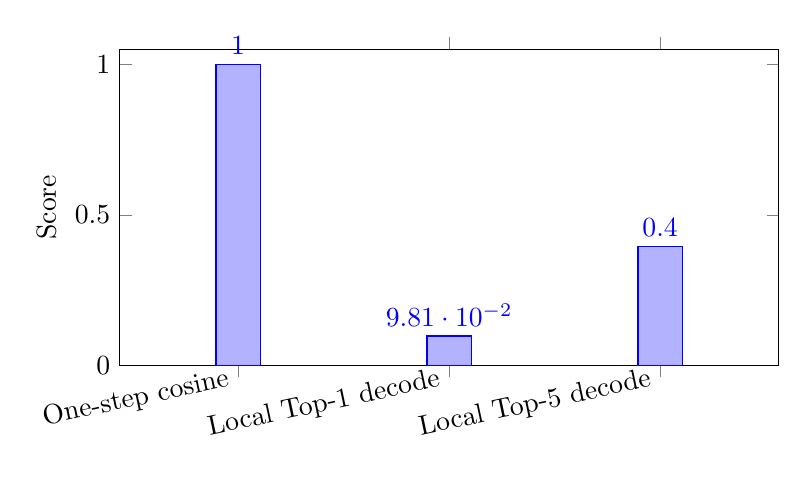
\begin{tikzpicture}
\begin{axis}[
    ybar,
    bar width=16pt,
    width=0.82\linewidth,
    height=5.6cm,
    ymin=0,
    ymax=1.05,
    ylabel={Score},
    symbolic x coords={One-step cosine,Local Top-1 decode,Local Top-5 decode},
    xtick=data,
    xticklabel style={rotate=12, anchor=east},
    nodes near coords,
    enlarge x limits=0.28
]
\addplot coordinates {(One-step cosine,0.9989) (Local Top-1 decode,0.0981) (Local Top-5 decode,0.3959)};
\end{axis}
\end{tikzpicture}
\caption{Experiment 4's core message: latent geometry is nearly perfect while exact decode remains much weaker.}
\label{fig:latent-gap}
\end{figure}

\subsection{Experiment 5: integrated memory--workspace--verification pipeline}
\begin{table}[t]
    \centering
    \caption{Integrated literature-synthesis pipeline over the same eight abstracts used in Experiment 2.}
    \begin{tabular}{lccc}
        \toprule
        Condition & Prompt load & Schema pass rate & Retrieval overlap \\
        \midrule
        Transcript-only & 62,536 & 0.625 & 0.000 \\
        Memory+Workspace & 25,081 & 0.875 & 0.625 \\
        Full integrated pipeline & 25,310 & 1.000 & 0.750 \\
        \bottomrule
    \end{tabular}
    \label{tab:integrated}
\end{table}

The integrated loop addresses the strongest structural critique of the previous draft: the modules are no longer evaluated only in isolation. Transcript-only execution both bloats prompt load and silently commits malformed notes, yielding a schema pass rate of just 0.625. Adding memory and bounded workspace cuts prompt load by roughly 60\% and improves retrieval overlap, but still leaves silent schema failures. The full integrated pipeline preserves the low prompt load, improves retrieval overlap to 0.75, restores schema pass rate to 1.0, and flags two failed commits before they enter trusted state. This supports H5: the modules matter most when they interact.

\subsection{Experiment 6: architectural comparison for latent state prediction}
\begin{table}[t]
    \centering
    \caption{Architectural comparison on the sequential latent transition task. We implement a minimal LRU as a tractable proxy for selective-scan state-space architectures; full Mamba requires hardware-aware CUDA kernels unavailable on Apple Silicon.}
    \begin{tabular}{lcccccc}
        \toprule
        Model & Params & Train s & Cosine & Top-1 local & Top-5 local & H5 cosine \\
        \midrule
        Causal Transformer & 368,640 & 1.068 & 0.9985 & 0.0682 & 0.3127 & 0.9988 \\
        Minimal LRU & 199,040 & 0.657 & 0.9982 & 0.0737 & 0.3202 & 0.9987 \\
        MLP control & 659,840 & 0.352 & 0.9986 & 0.0640 & 0.3189 & 0.9988 \\
        \bottomrule
    \end{tabular}
    \label{tab:sequence-models}
\end{table}

Experiment 6 yields the right kind of honest result. On cosine similarity, all three architectures are nearly indistinguishable, which means a smooth geometric metric would hide the architectural story. On exact local decode, however, the minimal LRU slightly exceeds both the causal transformer and the non-sequential MLP while using fewer parameters than either. This supports H6 in a narrow but meaningful sense: for short bounded-state episodes, recurrent compression is at least competitive with causal self-attention and slightly better on the exact metric that matters for symbolic state recovery.

\section{Discussion}
Six conclusions emerge.

First, long-horizon memory retrieval is not a contest between lexical and dense methods in the abstract. On LoCoMo, lexical retrieval remains strong because benchmark questions hinge on exact evidence spans, named entities, and temporal details. Dense retrieval adds robustness under paraphrase, but hybridization is the reliable choice.

Second, bounded workspace state is worth measuring rather than merely praising. Reconstructing prompts from explicit state cuts cumulative context load by more than half while preserving the resulting artifact on a real-data workflow.

Third, the planning critique is now stronger and less fragile. The earlier version could have been dismissed as ``tiny model fails at greedy planning.'' That complaint loses force once the experiment is scaled to Qwen2.5-1.5B-Instruct and a 3-shot CoT prompt. Greedy planning still fails, which clarifies why: the key-door task requires maintaining a boolean latent fact --- whether the agent has already acquired the key --- across several steps. Surface-fluent next-token prediction, even with lightweight CoT scaffolding, conflates local plausibility with state-consistent action selection. Verification and explicit search are therefore not decorative add-ons; they are the mechanism that restores reliability.

Fourth, the integrated pipeline matters because reviewer skepticism about fragmented evaluation was fair. Testing modules one by one is not enough. The integrated literature-synthesis loop is still lightweight, but it now shows all three active components interacting: memory retrieval changes which prior note is surfaced, bounded workspace changes the scaling law of prompt construction, and verification blocks malformed state updates before they become trusted memory.

Fifth, the latent world-model result is useful precisely because it is limited. Predicting next-state embeddings is geometrically easy, but exact decode remains weak. For agents that must eventually commit symbolic state, latent prediction cannot be the whole story.

Finally, the architectural comparison suggests that state-tracking problems should not be evaluated only through high-level smooth metrics. On short sequences the transformer is competitive, but the minimal recurrent proxy slightly wins on exact local decode while using fewer parameters. That does not prove state-space models are universally better; it does suggest that bounded-workspace agents deserve architectures whose inductive bias is closer to persistent hidden state than to quadratic attention over an ever-longer transcript.

\section{Limitations}
This paper still has important limits.
\begin{itemize}
    \item We do not train or fine-tune a real V-JEPA or VL-JEPA model. The latent dynamics experiment is an embedding-space baseline, not a claim of frontier-scale world-model training.
    \item The planning environment is symbolic, though the planners are real open-weight LMs. The result should be read as an architectural stress test, not as a benchmark of general planning competence.
    \item The integrated pipeline experiment uses a deterministic schema verifier rather than a learned or LLM-based judge; real agent verification is harder.
    \item The LRU implementation is a minimal proxy and does not use selective scan or hardware-aware kernels; results may not transfer to production state-space systems.
    \item CoT planning is evaluated on a single 3-shot template; prompt sensitivity is not ablated.
    \item The strongest empirical evidence in the paper is for memory, bounded state, and verification. The world-model component remains diagnostic rather than the dominant contribution.
\end{itemize}

These limitations are acceptable only if they are stated plainly. The paper is strongest as a systems argument with disciplined small-scale evidence, not as a claim of state-of-the-art agent performance.

\section{Conclusion}
The interesting question is no longer whether language models can be wrapped in tools. They can. The harder question is what additional machinery is necessary for agents to remain competent over long horizons. The experiments here point to a consistent answer. Memory should be persistent and hybrid. Prompt state should be bounded and reconstructed from workspace. Planning should be verifier-mediated rather than delegated to greedy decoding. Latent predictive state is useful, but only as one component inside a broader architecture that still respects exact commitments.

That is the paper's main claim. Not that one tiny model solves long-horizon autonomy, and not that world models alone magically fix agents. Rather, robust agents emerge when language is treated as an interface layered over memory, bounded state, prediction, and verification. The evidence is still small-scale, but it is now broad enough, integrated enough, and concrete enough to argue with.

\bibliographystyle{plainnat}
\bibliography{references}

\end{document}
